\section{Practical Constructions of Symmetric-Key Primitives}
\subsection*{Block Cipher}
Definition: Fixed input size strong PRP\\
$F:\{0,1\}^{n} \times \{0,1\}^{\ell}\rightarrow \{0,1\}^{\ell}$
\begin{itemize}
    \item $n$ - key size
    \item $\ell$ - block size
    \item $n$ and $\ell$ are both fixed
    \item Should take (approximately) $2^n$ time to attack
\end{itemize}

Avalanche Effect: Small change in input must affect every bit of output\\

Confusion-Diffusion  Paradigm
\begin{itemize}
    \item Confusion: $F_k(x)=f_1(x_1)||f_2(x_2)||\cdots||f_{16}(x_16)$
    \begin{itemize}
        \item $|x_i|$ = 8 bits
        \item $f_i$ can be a random permutation on 8 bits
        \item Goal: Introduce random local changes
    \end{itemize}
    \item Diffusion: Shuffle the bits using a mixing permutation
    \begin{itemize}
        \item This just moves bits around
        \item Goal: Spread confusion across all 128 bits
    \end{itemize}
    \item  Repeat many times
\end{itemize}

\subsection*{Feistel Networks}
Evaluating round $i$:
\begin{itemize}
    \item Split input in half: $L_{i-1}||R_{i-1}$
    \item $L_i=R_{i-1}$
    \item $R_i=L_{i-1}\oplus f_i(R_{i-1})$
\end{itemize}
Inverting round $i$:
\begin{itemize}
    \item Set $R_{i-1}=L_{i}$
    \item Set $L_{i-1}=R_i\oplus f_i(R_{i-1})$
\end{itemize}
Round Functions:
\begin{itemize}
    \item Each round has function $f_i$
    \item $f_i$ does not have to be invertible
    \item Usually $f_i$ derived from global public $f$ and round key $k_i$
\end{itemize}
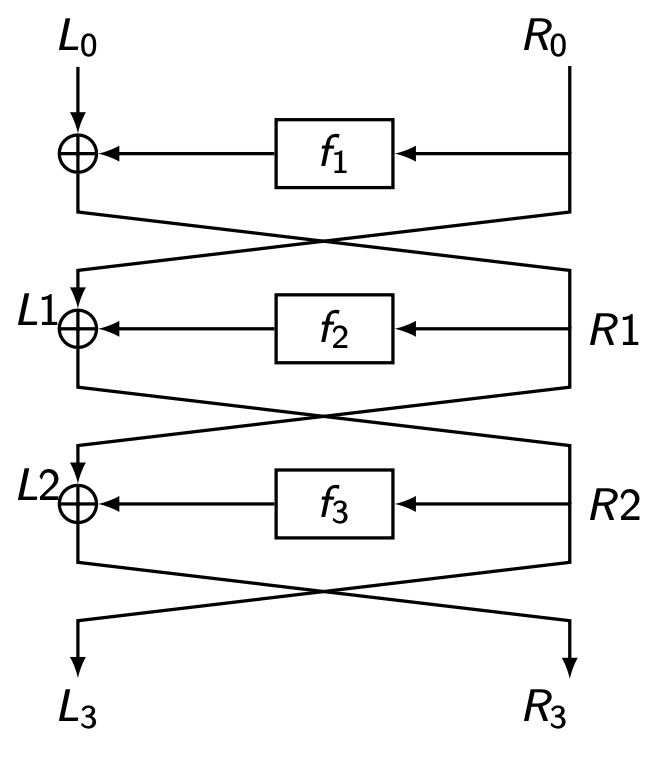
\includegraphics[width=\columnwidth]{Feistel.png}

\subsection*{SPN}
Repeat following for many rounds:
\begin{enumerate}
    \item Key mixing: Set $x=x\oplus k_i$
    \item Substitution: $x=S_1(x_1)||\cdots||S_8(x_8)$
    \item Permutation: Permute bits of $x$
\end{enumerate}
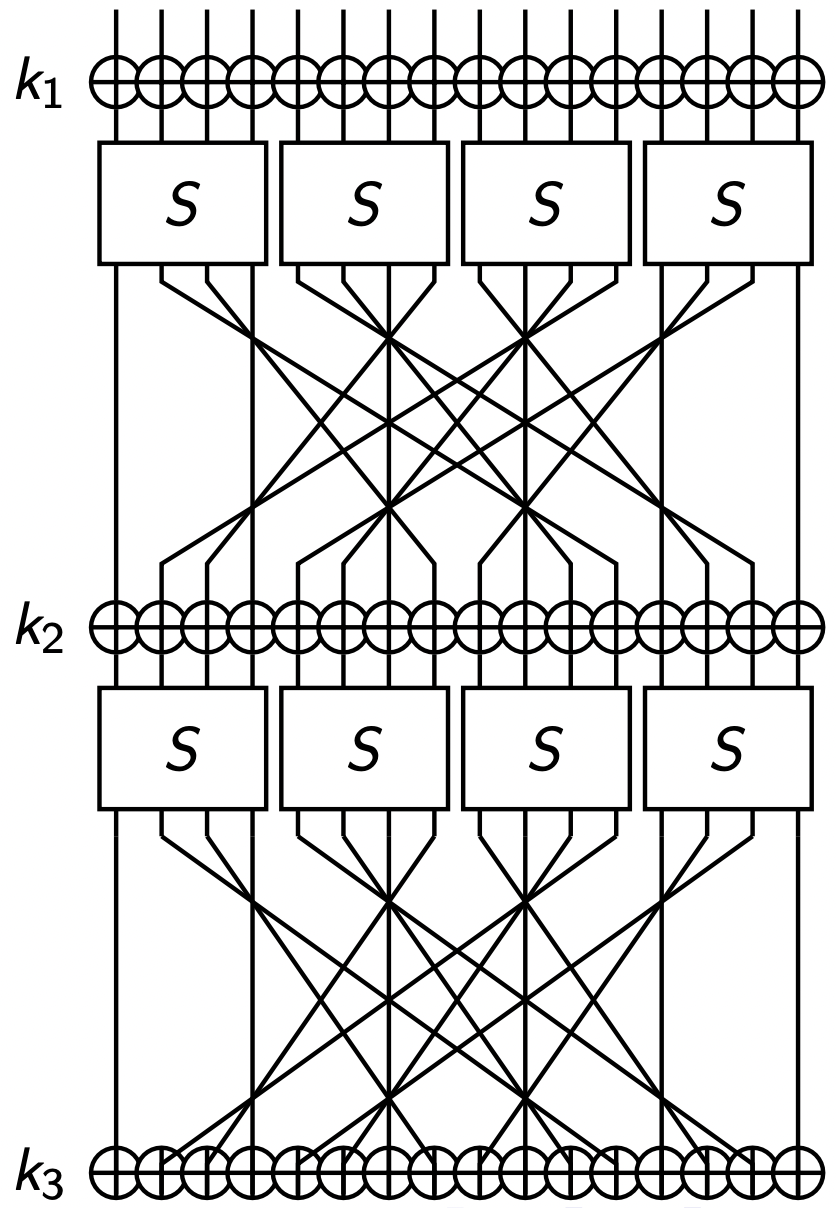
\includegraphics[width=\columnwidth]{SPN.png}

\subsection*{Data Encryption Standard(DES)}
\begin{itemize}
    \item Developed in 1970s by IBM + NSA
    \item $16$-round Feistel network with $\ell = 64$ (block length) and $n = 56$ (key length)
\end{itemize}
DES Key Schedule: Choosing round keys $k_i$ from master key $k$
\begin{itemize}
    \item $k\in \{0,1\}^{56},k_i\in \{0,1\}^{48}$
    \item Each $k_i$ is a subset of bits of $k$
    \item Which bits chosen in each round is public
\end{itemize}
DES Mangler Function:
\begin{itemize}
    \item $f_i(R)=\hat{f}(k_i,R),k_i\in \{0,1\}^{48},R\in \{0,1\}^{32}$
    \item Same $\hat{f}$ used in all $16$ rounds
    \item $\hat{f}$ is a substitution-permutation network (SPN)
    \item Extend $R$ to 48 bits by duplicating half of the bits of $R$: $R'=E(R)$
    \item Key mixing: $R''=R'\oplus k_i$
    \item Substitution\begin{enumerate}
        \item Break $R''$ into 8 blocks of 6bits
        \item Pass each block through differenct S-box (6-bit to 4bit) (not invertible)
    \end{enumerate}
    \item Permutation: Apply mixing permutation to 32-bit output
\end{itemize}

\subsection*{3DES}
Triple encryption with 3 keys:\\
$F''_{k_1,k_2,k_3}(x)=F_{k_3}(F_{k_2}^{-1}(F_{k_1}(x)))$\\
Triple encryption with 2 keys:\\
$F''_{k_1,k_2}(x)=F_{k_1}(F_{k_2}^{-1}(F_{k_1}(x)))$\\
Both variants have $2^{2n}$ security (meet-in-the-middle)

\subsection*{Davies-Meyer}
Collision-resistant hash function from an ideal block-cipher:
$h(s,x)=F_s(x)\oplus x$